\documentclass{standalone}
\usepackage{tikz}
\usetikzlibrary{shapes.geometric, arrows.meta, positioning}

\tikzset{
    % Estilos básicos
    startstop/.style={rectangle, rounded corners, minimum width=3.5cm, minimum height=1cm, text centered, draw=blue!80!black, fill=blue!10, very thick},
    process/.style={rectangle, minimum width=3.5cm, minimum height=1cm, text centered, draw=purple!80!black, fill=purple!10, very thick},
    decision/.style={diamond, aspect=2, text centered, draw=red!80!black, fill=red!10, very thick},
    arrow/.style={thick, ->, >=Stealth}
}

\begin{document}

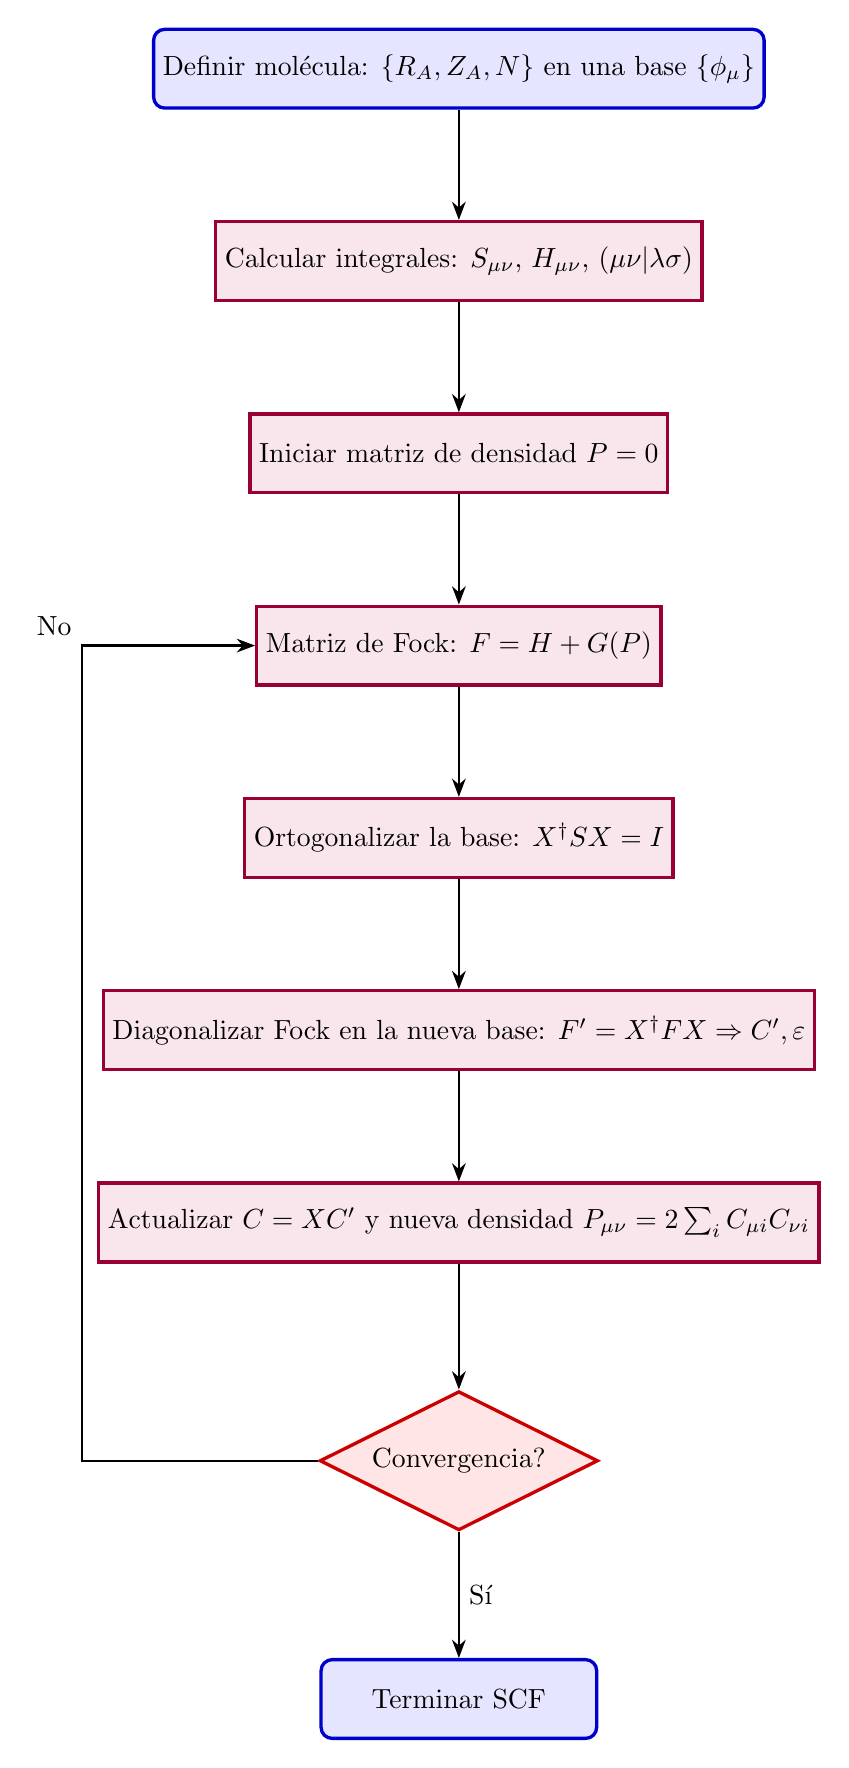
\begin{tikzpicture}[node distance=1.4cm]

% Nodos
\node (start) [startstop] {Definir molécula: $\{R_A, Z_A, N\}$ en una base $\{\phi_\mu\}$};
\node (integrals) [process, below=of start] {Calcular integrales: $S_{\mu\nu}$, \(H_{\mu\nu}\), $(\mu\nu|\lambda\sigma)$};
\node (guess) [process, below=of integrals] {Iniciar matriz de densidad $P=0$};
\node (fock) [process, below=of guess] {Matriz de Fock: $F = H + G(P)$};
\node (transform) [process, below=of fock] {Ortogonalizar la base: $X^\dagger S X = I$};
\node (diag) [process, below=of transform] {Diagonalizar Fock en la nueva base: $F' = X^\dagger F X \Rightarrow C', \varepsilon$};
\node (update) [process, below=of diag] {Actualizar $C = X C'$ y nueva densidad $P_{\mu\nu} = 2\sum_i C_{\mu i}C_{\nu i}$};
\node (conv) [decision, below=of update, yshift=-0.2cm] {Convergencia?};
\node (end) [startstop, below=of conv, yshift=-0.2cm] {Terminar SCF};

% Flechas
\draw [arrow] (start) -- (integrals);
\draw [arrow] (integrals) -- (guess);
\draw [arrow] (guess) -- (fock);
\draw [arrow] (fock) -- (transform);
\draw [arrow] (transform) -- (diag);
\draw [arrow] (diag) -- (update);
\draw [arrow] (update) -- (conv);
\draw [arrow] (conv) -- node[right]{Sí} (end);
\draw [arrow] (conv.west) -| ++(-3,0) |- node[above left]{No} (fock.west);

\end{tikzpicture}

\end{document}
